%%{{{
\documentclass{jsarticle}

% For code
\usepackage{moreverb}

% rendeing with dvipdfmx
\usepackage[dvipdfmx]{graphicx}

% 日本語での栞の文字化けを防ぐ
\usepackage{atbegshi}
\ifnum 42146=\euc"A4A2 \AtBeginShipoutFirst{\special{pdf:tounicode EUC-UCS2}}\else
\AtBeginShipoutFirst{\special{pdf:tounicode 90ms-RKSJ-UCS2}}\fi

\usepackage[dvipdfmx]{hyperref}

% floating image
\usepackage{float}

% ams series
\usepackage{amsmath}
\usepackage{amssymb}
\usepackage{amsthm}
\usepackage{ascmac}

% otf font
\usepackage{otf}

% 改ページの許可
\allowdisplaybreaks[1]

% definition, theorem
\theoremstyle{definition}
\newtheorem{theorem}{定理}
\newtheorem*{theorem*}{定理}
\newtheorem{definition}[theorem]{定義}
\newtheorem*{definition*}{定義}
\renewcommand\proofname{\bf 証明}

% "\vector{a}" でベクトル
\def\vector#1{\mbox{\boldmath \(#1\)}}

\hypersetup{breaklinks=true,
            bookmarks=true,
            pdfauthor={早稲田大学先進理工学研究科 物理学及応用物理学専攻 山崎研究室修士1年 藤本將太郎(5315A059)},
            pdftitle={非平衡系物理学特論レポート課題},
            colorlinks=true,
            citecolor=black,
            urlcolor=black,
            linkcolor=black,
            pdfborder={0 0 0}}
\urlstyle{same}  % don't use monospace font for urls

\title{非平衡系物理学特論レポート課題}
\author{早稲田大学先進理工学研究科 物理学及応用物理学専攻 山崎研究室修士1年
藤本將太郎(5315A059)}
\date{2016/01/21}
%}}}
\begin{document}

\setcounter{section}{-1}
\section{レポート課題}

\begin{enumerate}
\def\labelenumi{\arabic{enumi}.}
\itemsep1pt\parskip0pt\parsep0pt
\item
  DLAのプログラムを作成し、得られたDLAパターンのフラクタル次元を求めよ。
\item
  1次元ブラウン曲線でできた時系列をPCで作成し、得られた時系列のハースト指数を求めよ。
\end{enumerate}

\section{DLAパターンのフラクタル次元}

DLA(Diffusion Limited
Aggregation:拡散律速凝集)によって作られるパターンのフラクタル次元を,回転半径法によって求める。

DLAパターンの作成について,まず,正方格子状の格子点を考え,その原点を1つの粒子が占有している状態をスタートとする。
次に中心から距離\texttt{R}の位置に一つの粒子を(ランダムに)配置し,この粒子は単位時間ステップごとに上下左右の4方向に等確率で移動するようなランダムウォークを行うとする。

プログラムの実行時間を短縮するために,粒子が\texttt{R + 2}より遠い位置に存在するときにはランダムウォークの歩幅\texttt{l}を大きくし,\texttt{l = r - (R + 2)}(\texttt{r}はDLAの中心から粒子までの距離)のようにする。
また,粒子が中心からあまりにも遠く(\texttt{r \textgreater{} 2R})離れてしまった際には,その粒子を取り除き,再度中心から距離\texttt{R}の円周上から新しい粒子を出発させる。

粒子がDLAクラスターのどれかと4辺のうちどこかで接触した際には,その時点でその粒子をDLAクラスターに取り込むことにする。
また,初期出発円(半径\texttt{R})の半径は,中心から最も遠い点までの距離$r_{\text{max}}$として$R = r_{\text{max}} + 2$とすることにする。
さらに,粒子が付着するごとに,回転半径$R_{g}$を求め,記録しておく。
回転半径は粒子の重さ1,クラスターを形成する粒子数$N$として
\[R_{g} = \sqrt{\frac{1}{N} \sum_{i=1}^{N} r_{i}^{2}}\]
のようにして求めることができる。

DLAパターンを作成するのには付録に示すPythonスクリプト(\texttt{DLA.py}[\ref{dla}])を使用した。

実際に粒子数$N=16384$個として作成したDLAパターンを図\ref{fig:f1}に示す。
ここで粒子の色の違いは,何番目にDLAパターンに取り込まれたかものかを表すものとなっている。

\begin{figure}[H]
  \begin{center}
    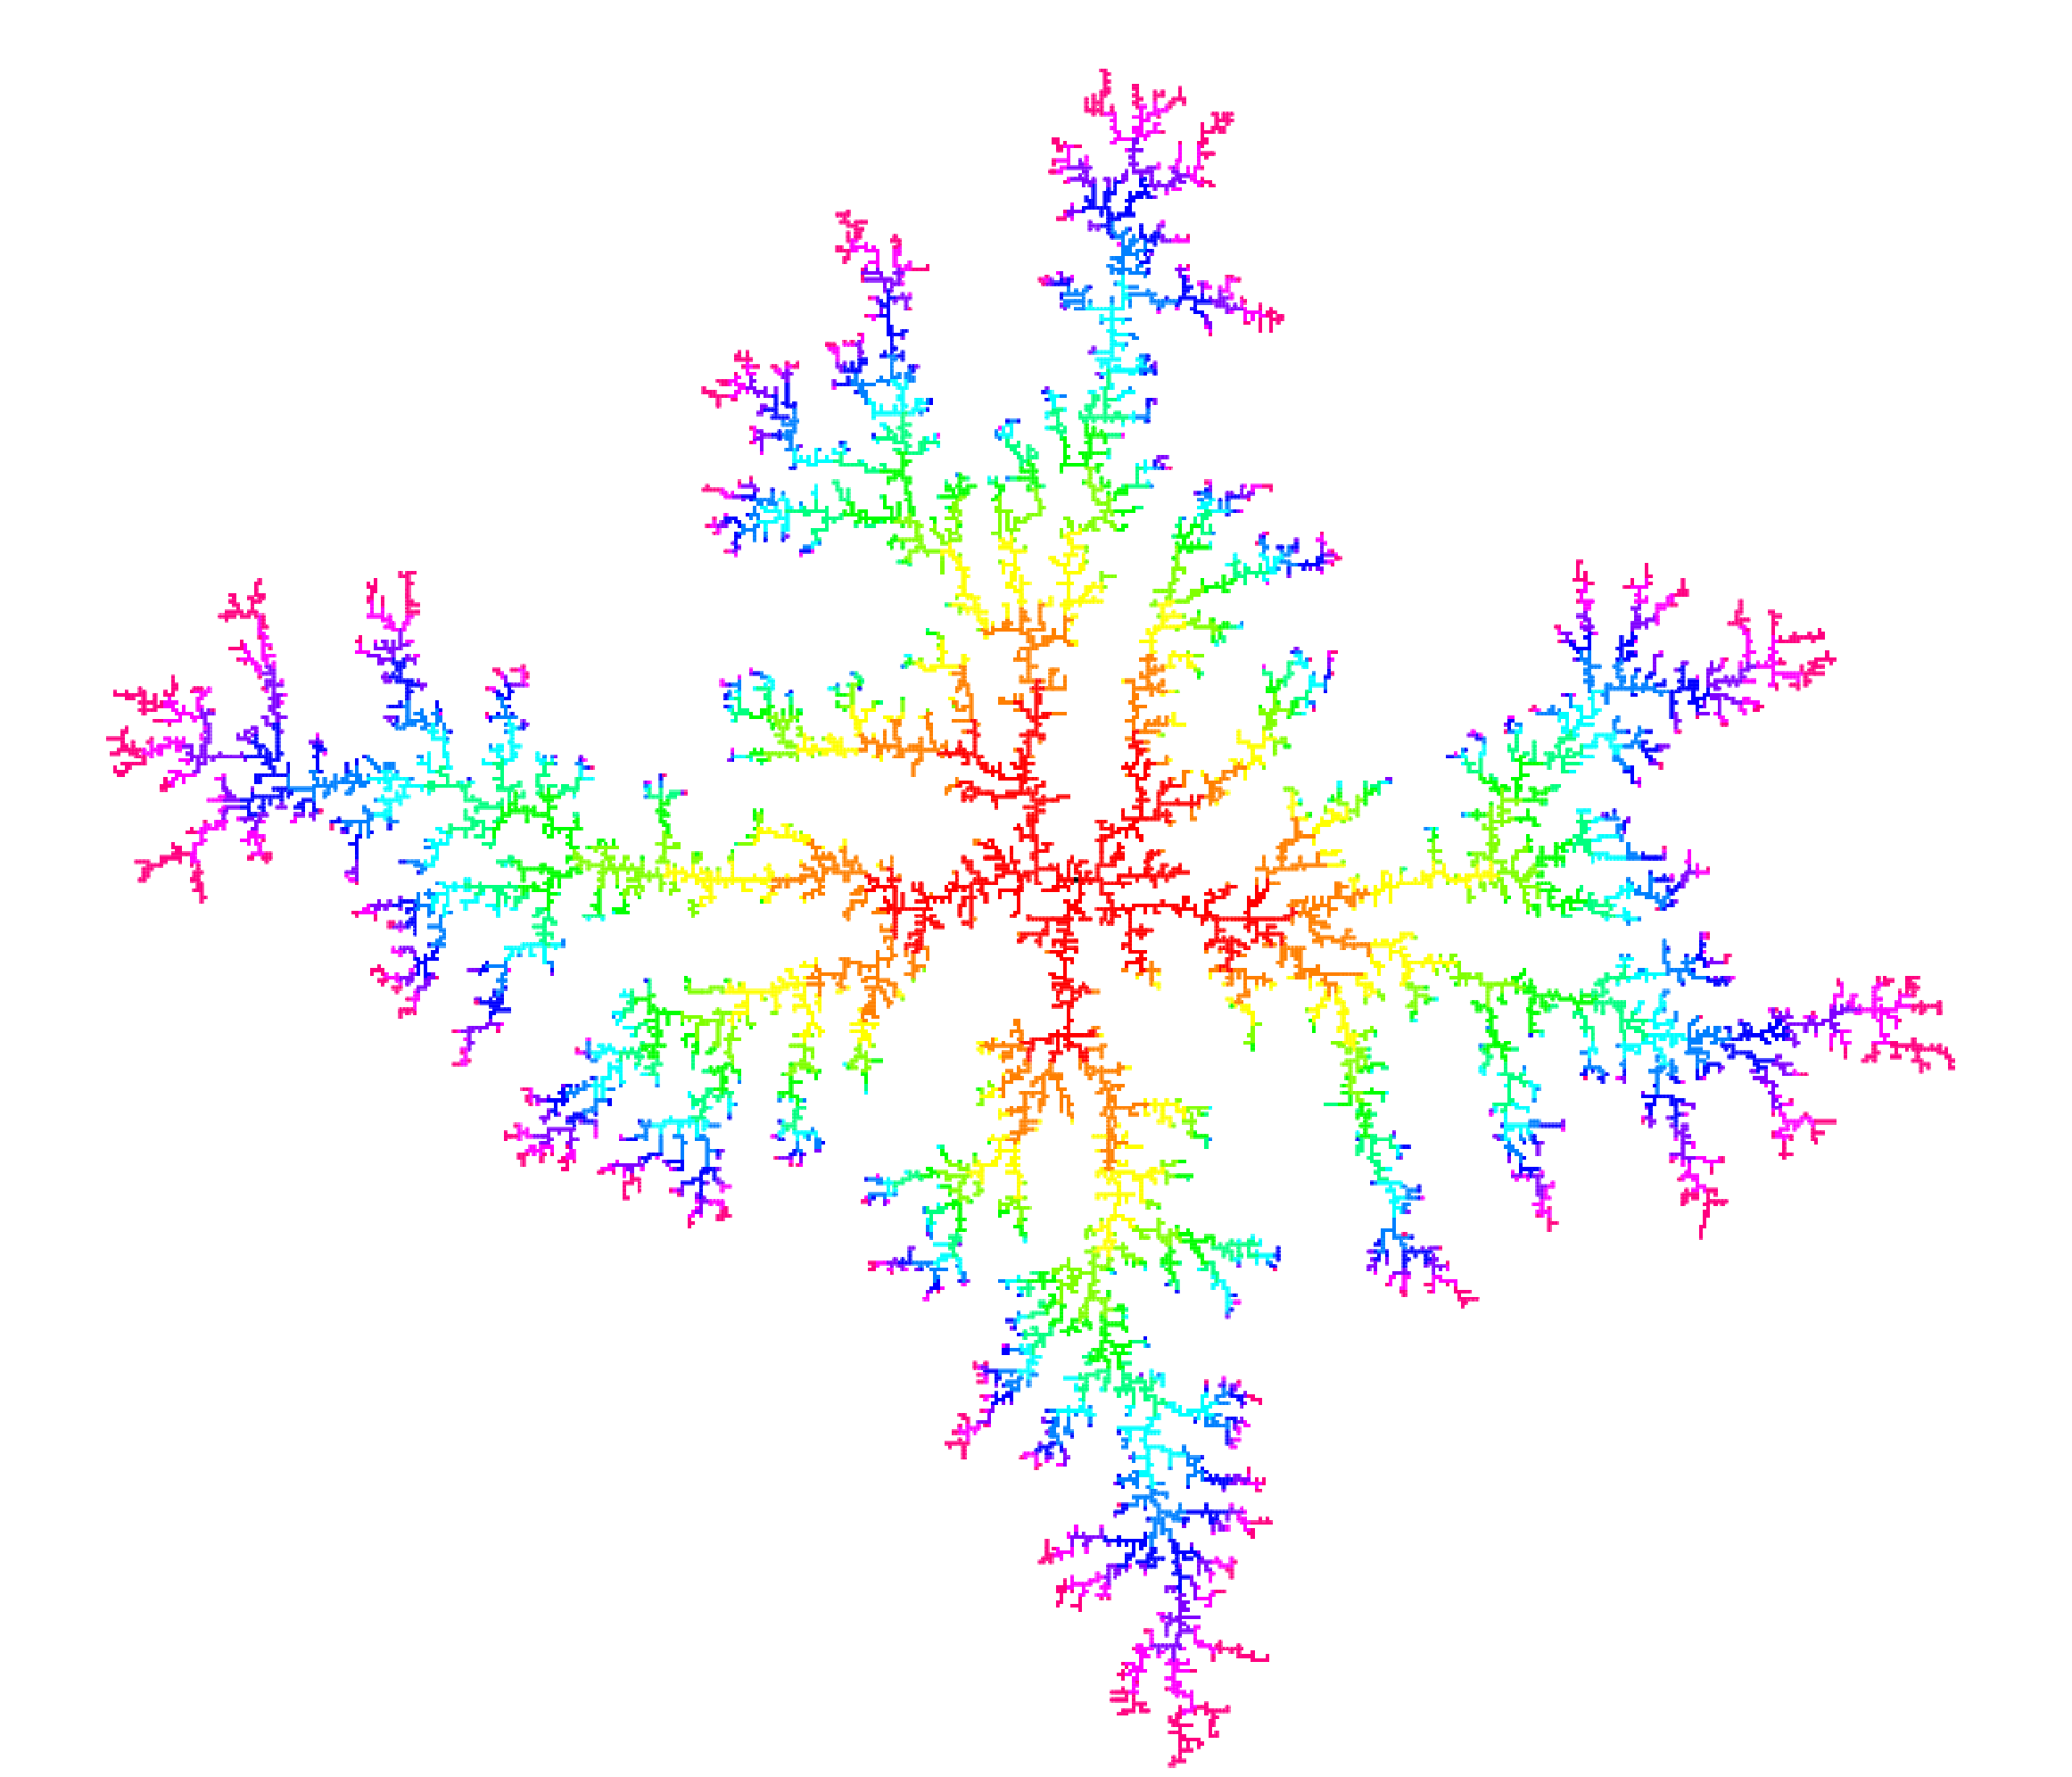
\includegraphics[width=\textwidth]{../img/screen_001.pdf}
    \caption{$N=16384$のときのDLAパターン}
    \label{fig:f1}
  \end{center}
\end{figure}

さて,図\ref{fig:f1}からもDLAパターンは自己相似的に見えるが,回転半径$R_{g}$と粒子数$N$の間に以下のようなスケール則が成り立つということが知られている。
\begin{eqnarray}
  N \sim R_{g}^{D}\label{e1}
\end{eqnarray}ここで$D$はフラクタル次元である。

したがって$R_{g}$と$N$を両対数グラフにプロットし,グラフ上で直線で近似すると,式(\ref{e1})からこの直線の傾きがフラクタル次元$D$に対応することが分かる(使用したプログラム: \texttt{SetParameter.py}[\ref{setparameter}], \texttt{fitting.py}[\ref{fitting}], \texttt{DLA.py}[\ref{dla}], \texttt{fractal\_dimension\_of\_DLA.py}[\ref{fractaldim}])。

実際に$N=16384$として作成したDLAパターンについて$R_{g}$と$N$を両対数グラフにプロットしたものを図\ref{fig:f2}に示す。
$N \ge 8$の範囲でフィッティングを行ったものがグラフ中の緑色で表した線分であり,この傾きは約$1.73$と求めることができた。
より大規模なシミュレーションによれば$D \simeq 1.71$となることが知られているが,今回のシミュレーションで得られたフラクタル次元と比較しても近い値であるので,本シミュレーションの結果もある程度の精度があると考えても良いだろう。

\begin{figure}[H]
  \begin{center}
    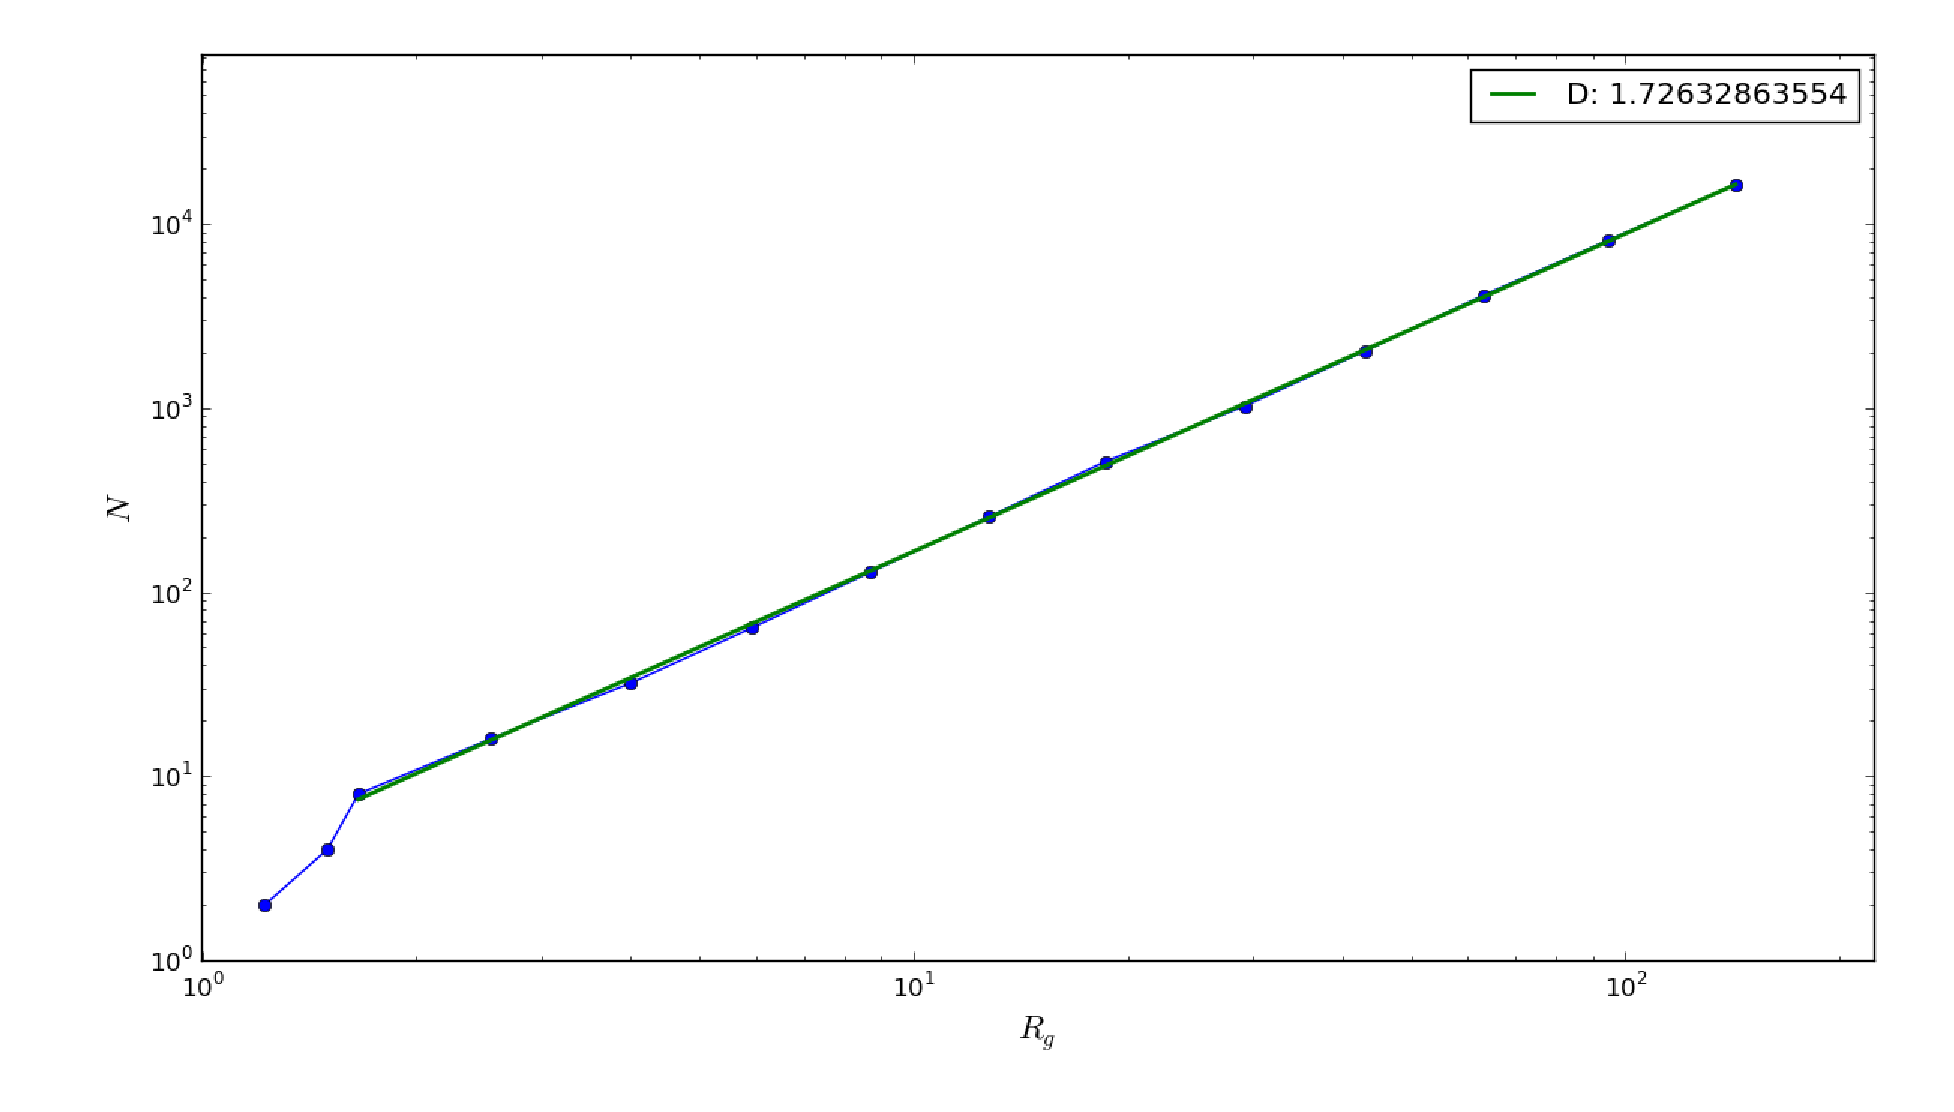
\includegraphics[width=\textwidth]{../img/fractal_dimension.pdf}
    \caption{回転半径$R_{g}$と$N$の間の関係}
    \label{fig:f2}
  \end{center}
\end{figure}

\section{1次元ブラウン曲線のハースト指数}

1次元ブラウン曲線$x(t)$は以下のように生成される時系列である:

\[x(t + 1) = x(t) + \xi(t)\]
\[\xi(t) = \left\{ \begin{array}{ll} +1 & (\text{with probability}\quad \frac{1}{2})\\
-1 & (\text{with probability}\quad \frac{1}{2}) \end{array}\right.\]

これをプログラム上で生成するために付録に示す\texttt{hurst.py}[\ref{hurst}]内の関数\texttt{brownian\_curve\_1d}を作成した。
この関数によって\texttt{N}ステップの時系列\texttt{X}が作成される。

実際にプログラムによって作成した1次元ブラウン曲線を図\ref{fig:f3}に示す。

\begin{figure}[H]
  \begin{center}
    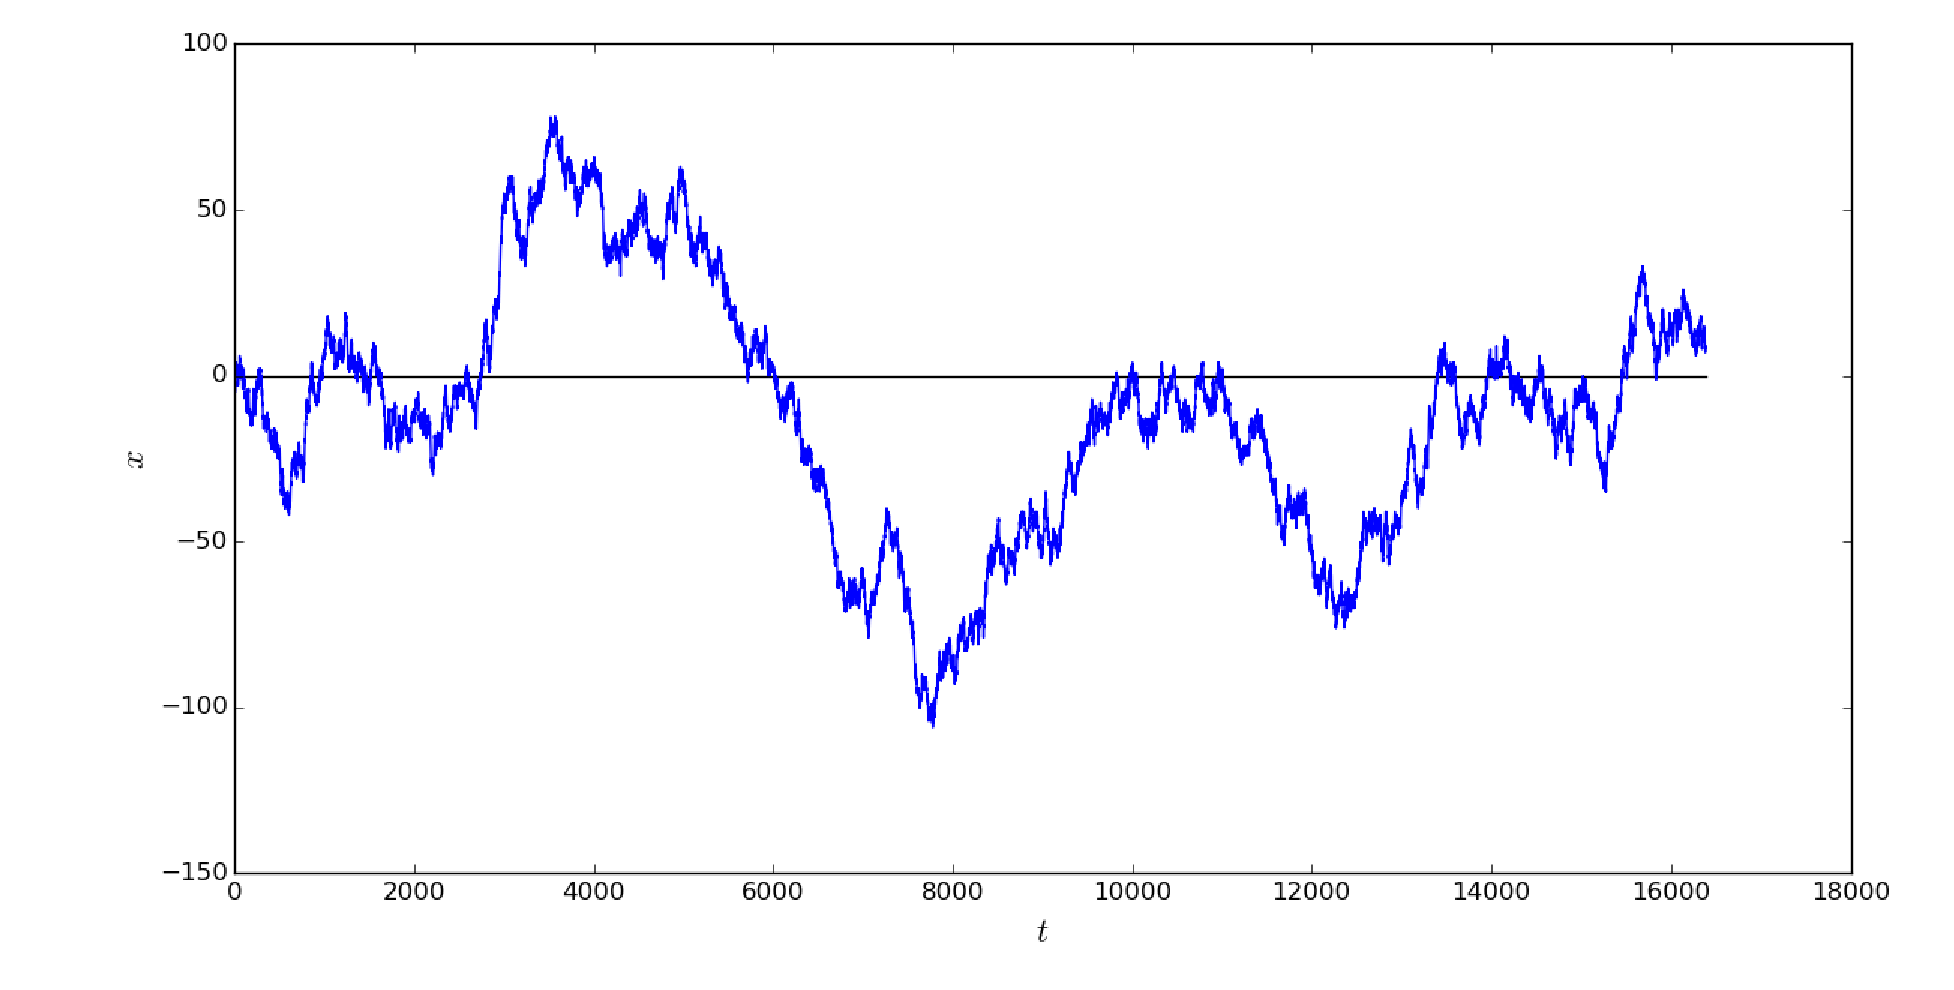
\includegraphics[width=\textwidth]{../img/brownian_motion.pdf}
    \caption{プログラムによって作成した1次元ブラウン曲線($T_{\text{max}} = 16383$)}
    \label{fig:f3}
  \end{center}
\end{figure}

ハースト指数はある時系列があったときに,その時間スケールと偏差の間で
\[t \rightarrow \varepsilon;\quad \sigma \rightarrow (\varepsilon \sigma)^{H}\]
のように縦と横で異なるスケール変換を行うことで$\sigma$の値が統計的に元の値と等しくなるときのこの$H$のことを意味する。

また,同じ意味であるが統計を取る時間$T$を決めてその範囲での偏差$\sigma_{x}(T)$を求め,これが
\[\sigma_{x}(T) \sim T^{H}\]
のような関係を満たすときの$H$をハースト指数と定義できる。

即ち,ある時系列について,統計を取る範囲$T$を変化させ,その時々に計算して得られる偏差$\sigma_{x}(T)$を記録し,横軸$T$,縦軸$\sigma_{x}$として両対数グラフにプロットし,直線で近似した時の傾きが$H$として求められるということが分かる。

実際に時系列についてハースト指数を計算するプログラムを作成した[\ref{hurst}]。
関数\texttt{calc\_hurst}によって,異なる$T$それぞれについて時系列全体を覆うようにサンプル範囲をスライドさせ,その時々に得られた偏差$\sigma$を平均することで,時系列のどの位置をサンプルとして選ぶかの依存性をなくした値を得ることができる。
このとき$T$が大きくなると当然取りうるサンプルの個数も少なくなることに注意が必要である。

このようにして各$T$について偏差$\sigma$の平均値を求め,これを両対数グラフにプロットしたものが図\ref{fig:f4}である。

\begin{figure}[H]
  \begin{center}
    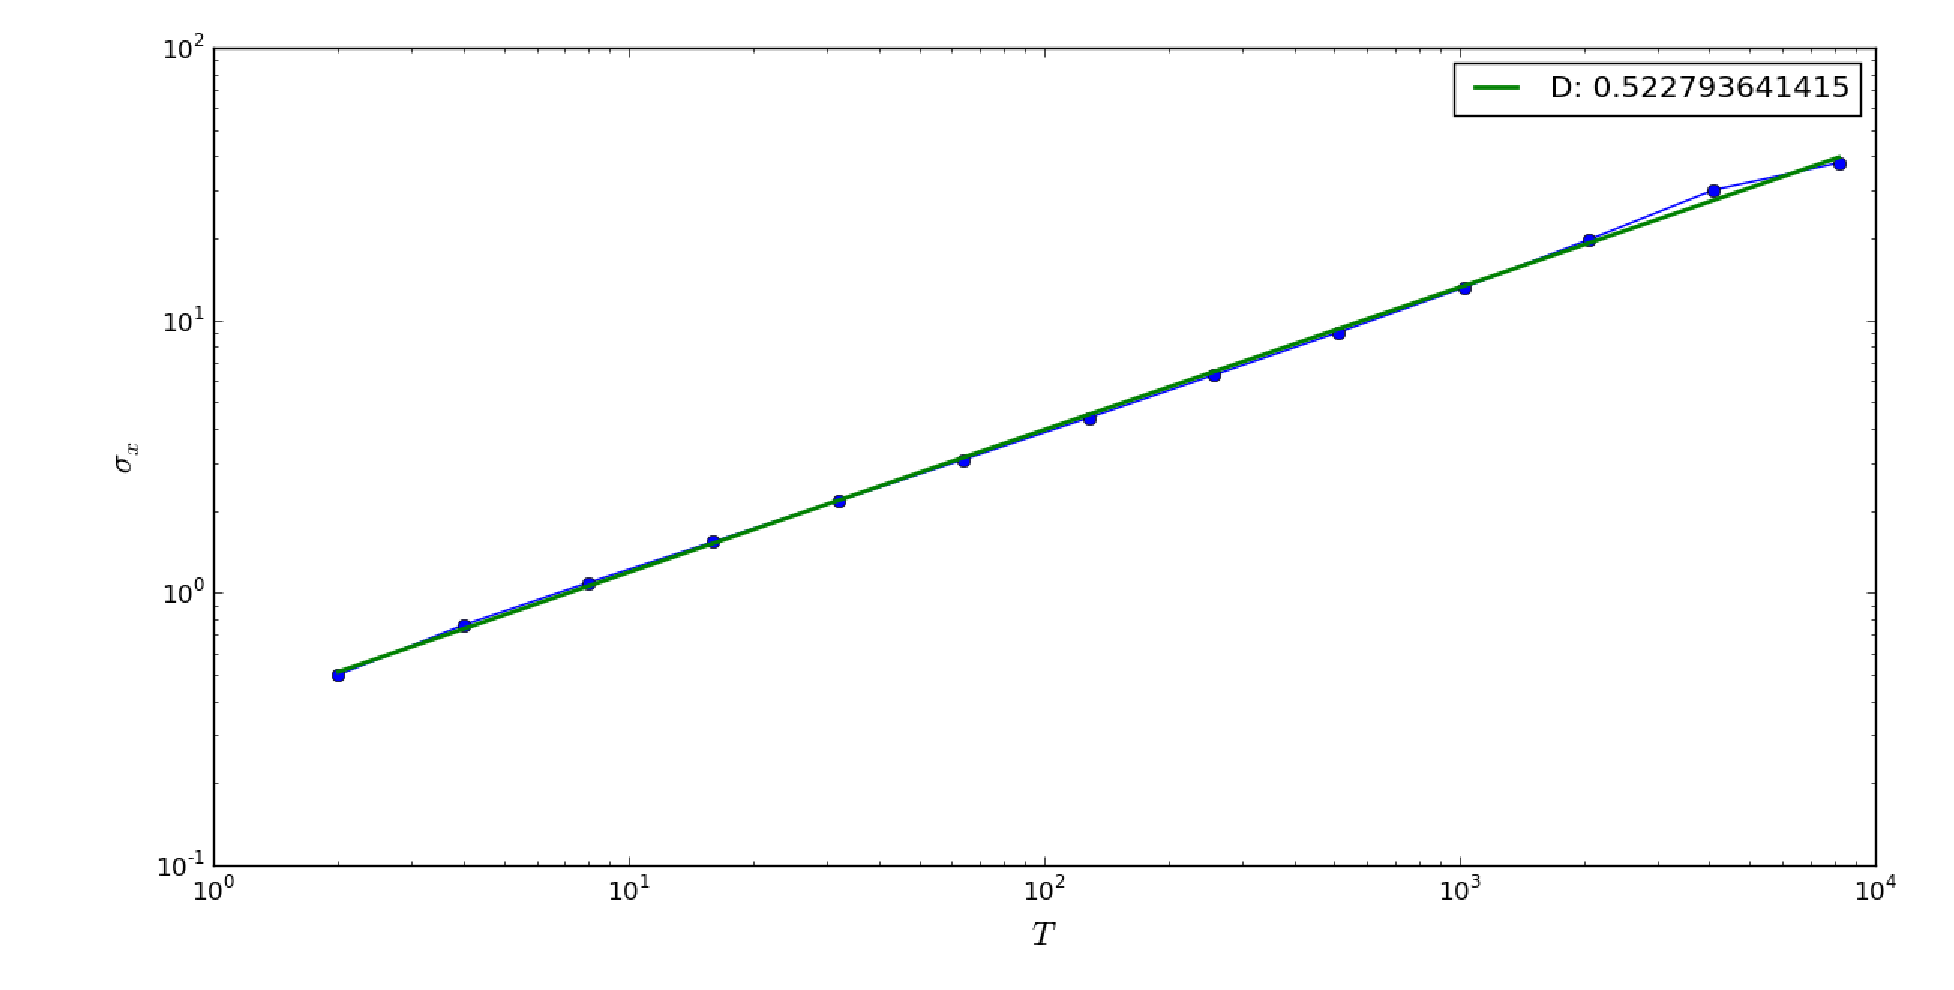
\includegraphics[width=\textwidth]{../img/hurst_exponent.pdf}
    \caption{$T$と$\sigma_{x}$の間の関係}
    \label{fig:f4}
  \end{center}
\end{figure}

この図からも直線で近似しても良さそうなことがわかり,実際にこれをフィッティングすると,緑色の線分のようになり,またその傾きは約0.523となった。
よく知られているように,1次元ブラウン曲線について$H = 0.5$であるので,これと比べても適切な値が得られていることが分かる。

\newpage
\section{付録}

\subsection{プログラムの実行用ダイアログを表示するスクリプト}\label{setparameter}
\texttt{SetParameter.py}
\listinginput{1}{../SetParameter.py}

\subsection{フィッティングを行うためのラッパー関数}\label{fitting}
\texttt{fitting.py}
\listinginput{1}{../fitting.py}

\subsection{DLAパターンを作成するスクリプト}\label{dla}
\texttt{DLA.py}
\listinginput{1}{../DLA.py}

\subsection{DLAのフラクタル次元を計算するための実行スクリプト}\label{fractaldim}
\texttt{fractal\_dimension\_of\_DLA.py}
\listinginput{1}{../fractal_dimension_of_DLA.py}

\subsection{1次元ブラウン曲線のハースト指数を求めるための実行スクリプト}\label{hurst}
\texttt{hurst.py}
\listinginput{1}{../hurst.py}

% % bib reference
% \bibliographystyle{junsrt}
% \bibliography{reference}

\end{document}
